\documentclass{ximera}

%\usepackage{todonotes}

\newcommand{\todo}{}

\usepackage{tkz-euclide}
\tikzset{>=stealth} %% cool arrow head
\tikzset{shorten <>/.style={ shorten >=#1, shorten <=#1 } } %% allows shorter vectors

\usepackage{tkz-tab}  %% sign charts
\usetikzlibrary{decorations.pathreplacing} 

\usetikzlibrary{backgrounds} %% for boxes around graphs
\usetikzlibrary{shapes,positioning}  %% Clouds and stars
\usetikzlibrary{matrix} %% for matrix
\usepgfplotslibrary{polar} %% for polar plots
\usetkzobj{all}
\usepackage[makeroom]{cancel} %% for strike outs
%\usepackage{mathtools} %% for pretty underbrace % Breaks Ximera
\usepackage{multicol}

\usepackage{polynom}



\usepackage[many]{tcolorbox}  %% for titled boxes
\newtcolorbox{xbox}[1]{%
    tikznode boxed title,
    enhanced,
    arc=0mm,
    interior style={white},
    attach boxed title to top center= {yshift=-\tcboxedtitleheight/2},
    fonttitle=\bfseries,
    colbacktitle=white,coltitle=black,
    boxed title style={size=normal,colframe=white,boxrule=0pt},
    title={#1}}


\usepackage{array}
\setlength{\extrarowheight}{+.1cm}   
\newdimen\digitwidth
\settowidth\digitwidth{9}
\def\divrule#1#2{
\noalign{\moveright#1\digitwidth
\vbox{\hrule width#2\digitwidth}}}





\newcommand{\RR}{\mathbb R}
\newcommand{\R}{\mathbb R}
\newcommand{\N}{\mathbb N}
\newcommand{\Z}{\mathbb Z}

%\renewcommand{\d}{\,d\!}
\renewcommand{\d}{\mathop{}\!d}
\newcommand{\dd}[2][]{\frac{\d #1}{\d #2}}
\newcommand{\pp}[2][]{\frac{\partial #1}{\partial #2}}
\renewcommand{\l}{\ell}
\newcommand{\ddx}{\frac{d}{\d x}}
\newcommand{\ddt}{\frac{d}{\d t}}

\newcommand{\zeroOverZero}{\ensuremath{\boldsymbol{\tfrac{0}{0}}}}
\newcommand{\inftyOverInfty}{\ensuremath{\boldsymbol{\tfrac{\infty}{\infty}}}}
\newcommand{\zeroOverInfty}{\ensuremath{\boldsymbol{\tfrac{0}{\infty}}}}
\newcommand{\zeroTimesInfty}{\ensuremath{\small\boldsymbol{0\cdot \infty}}}
\newcommand{\inftyMinusInfty}{\ensuremath{\small\boldsymbol{\infty - \infty}}}
\newcommand{\oneToInfty}{\ensuremath{\boldsymbol{1^\infty}}}
\newcommand{\zeroToZero}{\ensuremath{\boldsymbol{0^0}}}
\newcommand{\inftyToZero}{\ensuremath{\boldsymbol{\infty^0}}}



\newcommand{\numOverZero}{\ensuremath{\boldsymbol{\tfrac{\#}{0}}}}
\newcommand{\dfn}{\textbf}
%\newcommand{\unit}{\,\mathrm}
\newcommand{\unit}{\mathop{}\!\mathrm}
\newcommand{\eval}[1]{\bigg[ #1 \bigg]}
\newcommand{\seq}[1]{\left( #1 \right)}
\renewcommand{\epsilon}{\varepsilon}
\renewcommand{\iff}{\Leftrightarrow}

\DeclareMathOperator{\arccot}{arccot}
\DeclareMathOperator{\arcsec}{arcsec}
\DeclareMathOperator{\arccsc}{arccsc}
\DeclareMathOperator{\si}{Si}
\DeclareMathOperator{\proj}{proj}
\DeclareMathOperator{\scal}{scal}


\newcommand{\tightoverset}[2]{% for arrow vec
  \mathop{#2}\limits^{\vbox to -.5ex{\kern-0.75ex\hbox{$#1$}\vss}}}
\newcommand{\arrowvec}[1]{\tightoverset{\scriptstyle\rightharpoonup}{#1}}
\renewcommand{\vec}{\mathbf}
\newcommand{\veci}{\vec{i}}
\newcommand{\vecj}{\vec{j}}
\newcommand{\veck}{\vec{k}}
\newcommand{\vecl}{\boldsymbol{\l}}

\newcommand{\dotp}{\bullet}
\newcommand{\cross}{\boldsymbol\times}
\newcommand{\grad}{\boldsymbol\nabla}
\newcommand{\divergence}{\grad\dotp}
\newcommand{\curl}{\grad\cross}
%\DeclareMathOperator{\divergence}{divergence}
%\DeclareMathOperator{\curl}[1]{\grad\cross #1}


\colorlet{textColor}{black} 
\colorlet{background}{white}
\colorlet{penColor}{blue!50!black} % Color of a curve in a plot
\colorlet{penColor2}{red!50!black}% Color of a curve in a plot
\colorlet{penColor3}{red!50!blue} % Color of a curve in a plot
\colorlet{penColor4}{green!50!black} % Color of a curve in a plot
\colorlet{penColor5}{orange!80!black} % Color of a curve in a plot
\colorlet{fill1}{penColor!20} % Color of fill in a plot
\colorlet{fill2}{penColor2!20} % Color of fill in a plot
\colorlet{fillp}{fill1} % Color of positive area
\colorlet{filln}{penColor2!20} % Color of negative area
\colorlet{fill3}{penColor3!20} % Fill
\colorlet{fill4}{penColor4!20} % Fill
\colorlet{fill5}{penColor5!20} % Fill
\colorlet{gridColor}{gray!50} % Color of grid in a plot

\newcommand{\surfaceColor}{violet}
\newcommand{\surfaceColorTwo}{redyellow}
\newcommand{\sliceColor}{greenyellow}




\pgfmathdeclarefunction{gauss}{2}{% gives gaussian
  \pgfmathparse{1/(#2*sqrt(2*pi))*exp(-((x-#1)^2)/(2*#2^2))}%
}


%%%%%%%%%%%%%
%% Vectors
%%%%%%%%%%%%%

%% Simple horiz vectors
\renewcommand{\vector}[1]{\left\langle #1\right\rangle}


%% %% Complex Horiz Vectors with angle brackets
%% \makeatletter
%% \renewcommand{\vector}[2][ , ]{\left\langle%
%%   \def\nextitem{\def\nextitem{#1}}%
%%   \@for \el:=#2\do{\nextitem\el}\right\rangle%
%% }
%% \makeatother

%% %% Vertical Vectors
%% \def\vector#1{\begin{bmatrix}\vecListA#1,,\end{bmatrix}}
%% \def\vecListA#1,{\if,#1,\else #1\cr \expandafter \vecListA \fi}

%%%%%%%%%%%%%
%% End of vectors
%%%%%%%%%%%%%

%\newcommand{\fullwidth}{}
%\newcommand{\normalwidth}{}



%% makes a snazzy t-chart for evaluating functions
%\newenvironment{tchart}{\rowcolors{2}{}{background!90!textColor}\array}{\endarray}

%%This is to help with formatting on future title pages.
\newenvironment{sectionOutcomes}{}{} 



%% Flowchart stuff
%\tikzstyle{startstop} = [rectangle, rounded corners, minimum width=3cm, minimum height=1cm,text centered, draw=black]
%\tikzstyle{question} = [rectangle, minimum width=3cm, minimum height=1cm, text centered, draw=black]
%\tikzstyle{decision} = [trapezium, trapezium left angle=70, trapezium right angle=110, minimum width=3cm, minimum height=1cm, text centered, draw=black]
%\tikzstyle{question} = [rectangle, rounded corners, minimum width=3cm, minimum height=1cm,text centered, draw=black]
%\tikzstyle{process} = [rectangle, minimum width=3cm, minimum height=1cm, text centered, draw=black]
%\tikzstyle{decision} = [trapezium, trapezium left angle=70, trapezium right angle=110, minimum width=3cm, minimum height=1cm, text centered, draw=black]


\title[Dig-In:]{A tale of three integrals}

\begin{document}
\begin{abstract}
  At this point we have three ``different'' integrals. 
\end{abstract}
\maketitle

At this point we have three different ``integrals.'' Let's see if we
can sort out the differences.

\section{Indefinite integrals}

An indefinite integral, also called an \dfn{antiderivative} computes
classes of functions:
\[
\int f(x) \d x = \text{``a class of functions whose derivative is $f$''}
\]
Here there are no limits of integration, and your answer will have a
``$+C$'' at the end. Pay attention to the notation:
\begin{image}
  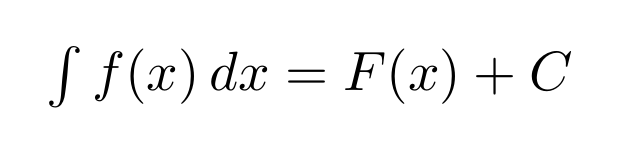
\begin{tikzpicture}[scale=2,every node/.style={transform shape}]
    \node at (0,0) {
      $\int f(x) \d x = F(x) + C$
      };
  \end{tikzpicture}
\end{image}
Where $F'(x) = f(x)$.
\begin{explanation}%%%BADBAD I would like no environment here.
  Indefinite integrals
  \wordChoice{\choice{have}\choice[correct]{do not have}} limits of
  integration, and they compute \wordChoice{\choice{signed
      area}\choice{an antiderivative}\choice[correct]{a class
      of antiderivatives}}.
\end{explanation}

\begin{question}
  Two students, say Devyn and Riley, are working with the following
  indefinite integral:
  \[
  \int \frac{2}{x\ln(x^2)}\d x
  \]
  Devyn computes the integral as
  \[
  \int \frac{2}{x\ln(x^2)}\d x = \ln|\ln|x^2|| + C
  \]
  and Riley computes the integral as
  \[
  \int \frac{2}{x\ln(x^2)}\d x = \ln|\ln|x|| + C.
  \]
  Which student is correct?
  \begin{multipleChoice}
    \choice{Devyn is correct}
    \choice{Riley is correct}
    \choice[correct]{Both students are correct}
    \choice{Neither student is correct}
  \end{multipleChoice}
  \begin{feedback}
    Both students are correct! The seeming discrepancy arises from the
    fact that the ``+C'' in each case is \textit{different}!
  \end{feedback}
\end{question}





\section{Accumulation functions}

An \dfn{accumulation function}, also called an \dfn{area function}
computes accumulated area:
\[
\int_a^x f(t) \d t = \text{``a function $F$ whose derivative is $f$''}
\]
This is a function of $x$ whose derivative is $f$, with the additional
property that $F(a)=0$.  Pay attention to the notation:
\begin{image}
  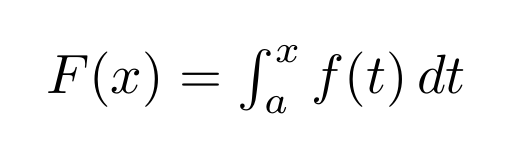
\begin{tikzpicture}[scale=2,every node/.style={transform shape}]
    \node at (0,0) {
      $F(x)=\int_a^x f(t) \d t$
      };
  \end{tikzpicture}
\end{image}
Where $F'(x) = f(x)$.
\begin{explanation}%%%BADBAD I would like no environment here.
  Accumulation functions \wordChoice{\choice[correct]{have}\choice{do
      not have}} limits of integration, and they compute
  \wordChoice{\choice{signed area}\choice[correct]{an antiderivative}\choice{a class of antiderivatives}}.
\end{explanation}
\begin{question}
  True or false: There exists a function $f$ such that 
  \[
  \int_0^x f(t) \d t = e^x
  \]
  \begin{prompt}
  \begin{multipleChoice}
    \choice{true}
    \choice[correct]{false}
  \end{multipleChoice}
  \begin{feedback}
    Let
    \[
    F(x) = \int_0^x f(t) \d t,
    \]
    this is an accumulation function and $F(0) = 0$, since no area is
    accumulated yet. However, $e^0 =1$. Hence there can be no such
    function $f$. On the other hand, there is a function $g$ with
     \[
     \int_0^x g(t) \d t = e^x-1
     \]
     namely, $g(x) = e^x$. This subtlety arises from the fact that an
     accumulation function
     \[
     F(x) = \int_a^x f(t) \d t
     \]
     gives a \textbf{specific} antiderivative of $f$, the one that
     when evaluated at $x=a$ is zero.
  \end{feedback}
  \end{prompt}
\end{question}










\section{Definite integrals}

A \dfn{definite integral} computes signed area:
\[
\int_a^b f(x) \d x = \text{``the signed area between the $x$-axis and $f$''}
\]
Here we always have limits of integration, both of which are
numbers. Moreover, definite integrals have definite values, the signed
area between $f$ and the $x$-axis. Pay attention to the notation:
\begin{image}
  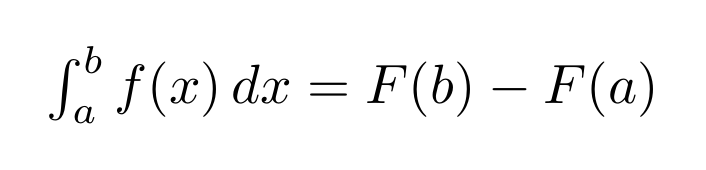
\begin{tikzpicture}[scale=2,every node/.style={transform shape}]
    \node at (0,0) {
      $\int_a^b f(x) \d x = F(b)-F(a)$
      };
  \end{tikzpicture}
\end{image}
Where $F'(x) = f(x)$.
\begin{explanation}%%%BADBAD I would like no environment here.
  Definite integrals \wordChoice{\choice[correct]{have}\choice{do
      not have}} limits of integration, and they compute
  \wordChoice{\choice[correct]{signed area}\choice{an antiderivative}\choice{a class of antiderivatives}}.
\end{explanation}

\begin{question}
  Consider
  \[
  f(x) =
  \begin{cases}
    -2  &\text{if $x< 1$,}\\
    2 &\text{if $x\ge 1$.}
  \end{cases}
  \]
  If we compute an antiderivative of $f$, we find
  \[
  F(x) =
  \begin{cases}
    -2x  &\text{if $x< 1$,}\\
    2x &\text{if $x\ge 1$.}
  \end{cases}
  \]
  Is it correct to say
  \begin{align*}
    \int_0^1 f(x) \d x &= \eval{F(x)}_0^1 \\
    &=F(1) - F(0)\\
    &=2 ?
  \end{align*}
  \begin{multipleChoice}
    \choice{yes}
    \choice[correct]{no}
  \end{multipleChoice}
  \begin{feedback}
    Perhaps the first thing to do would be to attempt to analyze this
    geometrically. Here we see our function and the signed area
    computed by the integral:
    \begin{image}
      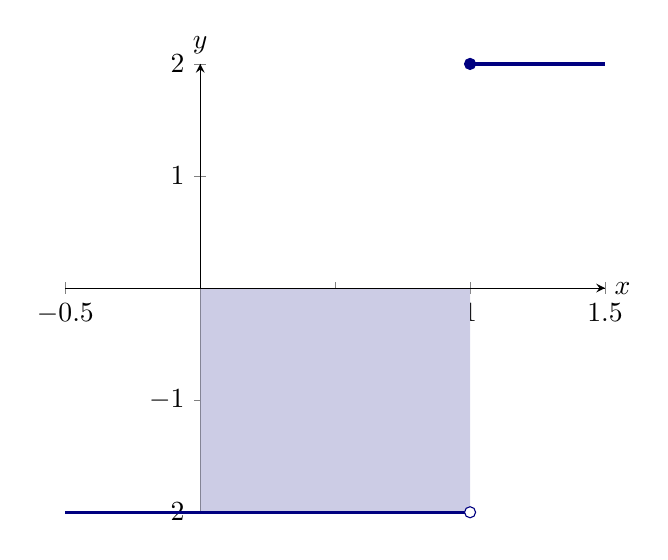
\begin{tikzpicture}
	\begin{axis}[
            domain=-.5:1.5,
            axis lines =middle, xlabel=$x$, ylabel=$y$,
            every axis y label/.style={at=(current axis.above origin),anchor=south},
            every axis x label/.style={at=(current axis.right of origin),anchor=west},
            clip=false,
            %axis on top,
          ]
          \addplot [draw=none,
            fill=fillp, domain=0:1] {-2} \closedcycle;
          \addplot [textColor, very thin, domain=(0:1.5)] {0}; % puts the axis back, axis on top clobbers our open holes
          \addplot [textColor, very thin] plot coordinates {(0,0) (0,2)}; % puts the axis back, axis on top clobbers our open holes
	  \addplot [very thick, penColor, domain=(-.5:1)] {-2};
          \addplot [very thick, penColor, domain=(1:1.5)] {2};
          \addplot[color=penColor,fill=penColor,only marks,mark=*] coordinates{(1,2)};  %% closed hole          
          \addplot[color=penColor,fill=background,only marks,mark=*] coordinates{(1,-2)};  %% open hole
        \end{axis}
      \end{tikzpicture}
    \end{image}
    From the graph above, we can see that
    \[
    \int_0^1 f(x) \d x =-2.
    \]
    So now the question is, ``what went wrong'' above? In this case
    our function $f$ is \textbf{not} continuous! For The Fundamental
    Theorem of Calculus to apply, the integrand \textbf{must} be
    continuous on the interval that one is integrating on. If this is
    not the case, the fundamental theorem may or may not yield valid
    results.
  \end{feedback}
\end{question}

\end{document}
